\documentclass[12pt]{article}
\usepackage{enumitem}
\usepackage{setspace}
\usepackage{graphicx}
\usepackage{subcaption}
\usepackage{amsmath, amsthm}
\usepackage{booktabs}
\RequirePackage[colorlinks]{hyperref}
\usepackage[lined,boxed,linesnumbered,commentsnumbered]{algorithm2e}
\usepackage{xcolor}
\usepackage{listings}
\lstset{basicstyle=\ttfamily,
  showstringspaces=false,
  commentstyle=\color{red},
  keywordstyle=\color{blue}
}

% Margins
\topmargin=-0.45in
\evensidemargin=0in
\oddsidemargin=0in
\textwidth=6.5in
\textheight=9.0in
\headsep=0.25in

\linespread{1.1}

% Commands
\newenvironment{solution}
  {\begin{proof}[Solution]}
  {\end{proof}}

\title{CSE6250: Big Data Analytics in Healthcare \\ Homework 1}
\author{Jimeng Sun}
\date{Deadline: Sep 1, 2019 Anytime on Earth\\ (i.e., 8am Sep 2, 2019, EST)}

\begin{document}

\maketitle
\begin{itemize}
\item You can use 2 days of late submission throughout the semester \textbf{ONLY for homeworks}.
\item Discussion is encouraged, but each student must write his/her own answers and explicitly mention any collaborators.
\item Each student is expected to respect and follow the \href{http://www.honor.gatech.edu/}{ GT Honor Code}. \textbf{We will apply anti-cheating software to check for plagiarism.} Any one who is flagged by the software will automatically receive 0 for the homework and be reported to the college.
\item Please type the submission with \LaTeX\ or Microsoft Word. We \textbf{will not} accept hand written submissions.
\item Please \textbf{do not change the filenames and function definitions} in the skeleton code provided, as this will cause the test scripts to fail and you will  receive no points in those failed tests. Built-in modules of python and the following libraries -  pandas, numpy, scipy, scikit-learn can be used. 
%\item Update the README.txt file in the folder to include the version of python you have used. 
\item It is your responsibility to make sure that all code and other deliverables are in the correct format and that your submission compiles and runs. We will not manually check your code (not feasible given the class size). Thus \textbf{non-runnable code in our test environment will directly lead to 0 score} without comments.
\end{itemize}

\section*{Overview}

Preparing the data, computing basic statistics and constructing simple models are essential steps for  data science practice. In this homework, you will use clinical data as raw input to perform \textbf{Mortality Prediction}. For this homework, \textbf{Python} programming will be required. See the attached skeleton code as a start-point for the programming questions. Also, you need to \textbf{make a single PDF file (\textit{homework1\_answer.pdf}) }of a compiled document for non-programming questions.



\section{CITI Certification  [10 points] }
During this course, we will be working with the MIMIC database. MIMIC, although de-identified, still contains detailed information regarding the clinical care of patients, and must be treated with appropriate care and respect. In order to obtain access, it is necessary to finish the MIMIC CITI program training provided by MIT and get the certificate.

\begin{enumerate}
\item Navigate to the website: \url{https://www.citiprogram.org/index.cfm?pageID=154&icat=0&ac=0}. Under Register, select ''Massachusetts Institute of Technology Affiliate'' as your organization affiliation (not ''independent learner'') and create your account with your \textbf{GT email address (required)}.
\item Follow the links to add a Massachusetts Institute of Technology Affiliates course. In the Human Subjects training category, select the \textbf{"Data or Specimens Only Research"} course
\item Complete the course and save your completion report, which lists all modules completed with dates and scores.

\end{enumerate}
\textit{Solution:} Please include your certificates named \textit{$Certificate\_ MIMIC.pdf$} as the submission format we provided at the end.\\

\section*{About Raw Data}
Navigate to \textit{homework1/data/train}. There are three CSV files which will be the input data in this homework. 

The data provided in \textit{$events.csv$} are event sequences. Each line of this file consists of a tuple with the format \textit{(patient\textunderscore id, event\textunderscore id, event\textunderscore description, timestamp, value)}. 

For example, 

\begin{lstlisting}[frame=single, language=bash]
1053,DIAG319049,Acute respiratory failure,2924-10-08,1.0
1053,DIAG197320,Acute renal failure syndrome,2924-10-08,1.0
1053,DRUG19122121,Insulin,2924-10-08,1.0
1053,DRUG19122121,Insulin,2924-10-11,1.0
1053,LAB3026361,Erythrocytes in Blood,2924-10-08,3.000
1053,LAB3026361,Erythrocytes in Blood,2924-10-08,3.690
1053,LAB3026361,Erythrocytes in Blood,2924-10-09,3.240
1053,LAB3026361,Erythrocytes in Blood,2924-10-10,3.470
\end{lstlisting}

\begin{itemize}
\item \textbf{patient\textunderscore id}: De-identified patient identiers. For example, the patient in the example above has patient id 1053. 
\item \textbf{event\textunderscore id}: Clinical event identifiers. For example, DRUG19122121 means that a drug with RxNorm code as 19122121 was prescribed to the patient. DIAG319049 means the patient was diagnosed of disease with SNOMED code of 319049 and LAB3026361 means that the laboratory test with a LOINC code of 3026361 was conducted on the patient.
\item $\textbf{event\textunderscore description}$: Shows the description of the clinical event. For example, DIAG319049 is the code for Acute respiratory failure and DRUG19122121 is the code for Insulin. 
\item \textbf{timestamp}: the date at which the event happened. (Here the timestamp is not a real date.)
\item \textbf{value}: Contains the value associated to an event. See Table~\ref{tbl:value} for the detailed description.
\end{itemize}

\begin{table}[th]
\centering
\begin{tabular}{@{}llp{4cm}l@{}}
\toprule
event type & sample event\textunderscore id & value meaning & example \\ \midrule
diagnostic code & DIAG319049 & diagnosed with a certain disease, value always be 1.0 & 1.0 \\
drug consumption  & DRUG19122121  & prescribed a certain medication, value will always be 1.0 & 1.0 \\
laboratory test & LAB3026361 & test conducted on a patient and its value & 3.690 \\ \bottomrule
\end{tabular}
\caption{Event sequence value explanation}
\label{tbl:value}
\end{table}

The data provided in \textit{mortality\textunderscore events.csv} contains the patient ids of only the deceased people. They are in the form of a tuple with the format \textit{(patient\textunderscore id, timestamp, label)}. For example,
\begin{lstlisting}[frame=single, language=bash]
37,3265-12-31,1
40,3202-11-11,1
\end{lstlisting}

The timestamp indicates the death date of a deceased person and a label of 1 indicates death. Patients that are not mentioned in this file are considered alive.

The \textit{event\textunderscore feature\textunderscore map.csv} is a map from an event\_id (SNOMED, LOINC and RxNorm) to an integer index. This file contains \textit{(idx, event\textunderscore id)} pairs for all event ids.

\section*{Python and dependencies}
In this homework, we will work on Python 3.6.5 environment. If you do not have a python distribution installed yet, we recommend installing \href{https://docs.continuum.io/anaconda/install}{Anaconda} (or miniconda) with Python 3.6.5. We provide \textit{homework1/environment.yml} which contains a list of libraries needed to set environment
for this homework. You can use it to create a copy of conda `environment' (\href{http://conda.pydata.org/docs/using/envs.html#use-environment-from-file}{http://conda.pydata.org/docs/using/envs.html\#use-environment-from-file}). If you already have your own Python development environment (it should be Python 3.6.5), please refer to this file to find necessary libraries, which is used to set the same coding/grading environment. \\

\noindent Alternatively, we have prepared the docker environment. You are highly encouraged to set the environment ready ASAP following the tutorials of this \href{http://sunlab.org/teaching/cse6250/fall2018/env/#setup-virtual-environment}{link}, which you might use often in later homework. Please also activate \textit{environment.yml} when needed in coding.


\section*{Running the tests}
Test cases are provided for every module in this homework and operate on a subset of the data. To run a test, execute the following commands from the base folder i.e. homework1. If any of the test cases fail, an error will be shown. For example to test the statistics computed, the following command should be executed: \\

\begin{lstlisting}[frame=single, language=bash]
nosetests tests/test_statistics.py --nologcapture
\end{lstlisting}

\noindent A single test can also be run using this syntax: \\    
%\textbf{nosetests tests/$<filename>$:$<test\_method>$}\\
\begin{lstlisting}[frame=single, language=bash]
nosetests tests/<filename>:<test_method> --nologcapture
\end{lstlisting}
Remember to use the right \textit{filename} and \textit{test\_method} in above command line. For more information about basic usage of nosetests, please refer to this \href{https://nose.readthedocs.io/en/latest/usage.html?highlight=#cmdoption--nologcapture}{LINK}

 \section{Descriptive Statistics [10 points]}
Before starting analytic modeling, it is a good practice to get descriptive statistics of the input raw data. In this section, you need to write code that computes various metrics on the data described previously. A skeleton code is provided to you as a starting point.

The definition of terms used in the result table are described below:
\begin{itemize}
\item \textbf{Event count}: Number of events recorded for a given patient. Note that every line in the input file is an event. 
\item \textbf{Encounter count}: Count of unique dates on which a given patient visited the hospital. All the events - DIAG, LAB and DRUG - should be considered as hospital visiting events.
\item \textbf{Record length}: Duration (in number of days) between the first event and last event for a given patient. \\
For example, if the first event is on 2014-05-21 and the last event is on 2014-05-24, the duration is 3 days. If a patient has only one event, the duration is 0.
\end{itemize}

\textbf{a.} Complete \textit{src/event\_statistics.py} to implement the required statistics.

Please be aware that \textbf{\color{red} you are NOT allowed to change the filename and any existing function declarations.} Only numpy, scipy, scikit-learn and other built-in modules of python will be available for you to use. The use of $pandas$ library is suggested. 

\textbf{b.} Use \textit{events.csv} and \textit{mortality\_events.csv} provided in \textbf{data/train} as input and fill Table~\ref{tbl:stat} with actual values. Include this table in \textit{homework1\_answer.pdf}\\

\begin{table}[th]
\centering
\begin{tabular}{@{}l|l|l|l@{}}
\toprule
Metric & Deceased patients & Alive patients & Function to complete \\ \hline
Event Count & & & event\_count\_metrics \\ 
1. Average Event Count &&& \\
2. Max Event Count  &&&\\
3. Min Event Count  &&&\\ \hline

Encounter Count & & & encounter\_count\_metrics \\ 
1. Average Encounter Count  &&&\\
2. Max Encounter Count  &&&\\
3. Min Encounter Count  &&&\\ \hline

Record Length & & & record\_length\_metrics \\ 
1. Average Record Length &&&\\
2. Max Record Length&&& \\
3. Min Record Length&&& \\ 
\bottomrule
\end{tabular}
\caption{Descriptive statistics for alive and dead patients}
\label{tbl:stat}
\end{table} 

\textbf{Deliverable: src/event\_statistics.py, homework1\_answer.pdf  [10 points]}

\section{Feature construction [30 points] }
It is a common practice to convert raw data into a standard data format before running real machine learning models. In this section, you will work on \textit{src/etl.py} file and implement the necessary python functions in this script. You will work with \textit{events.csv}, \textit{mortality\textunderscore events.csv} and \textit{event\textunderscore feature\textunderscore map.csv} files provided in \textbf{data/train} folder.  The use of $pandas$ library in this question is recommended. 
Listed below are a few concepts you need to know before beginning feature construction (for details please refer to lectures). 
\begin{center}
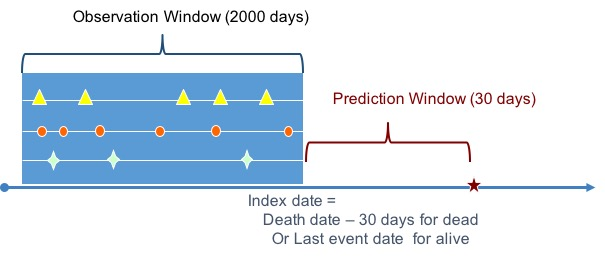
\includegraphics[width=.75\textwidth]{window.jpg}
\end{center}
\begin{itemize}
\item Observation Window: The time interval you will use to identify relevant events. Only events present in this window should be included while constructing  feature vectors. The size of observation window is 2000 days. 
\item Prediction Window: A fixed time interval that is to be used to make the prediction. Events in this interval should not be included in constructing feature vectors. The size of prediction window is 30 days. 
\item Index date: The day on which mortality is to be predicted. Index date is evaluated as follows:
\begin{itemize}
\item For deceased patients: Index date is 30 days prior to the death date (timestamp field) in \textit{data/train/mortality\textunderscore events.csv}. 
\item For alive patients: Index date is the last event date in \textit{data/train/events.csv} for each alive patient. 

\end{itemize}
\end{itemize}
Note: In the test\_etl.py test, please \textbf{be careful} the format of \textbf{trailing space and line breaks} issue we provide in the \textit{test\_feature\_order}. Adding a trailing blanks is not required in solution but adding it will not hurt grading. Line breaks are mandatory for grading. 

\textbf{Step - a.} Compute the index date [8 points]
\newline
Use the definition provided above to compute the index date for all patients. Complete the method \textit{$calculate\_index\_date$} provided in \textit{src/etl.py} . 
\newline

\textbf{Deliverable: \textit{src/etl.py, deliverables/etl\_index\_dates.csv}}
\newline

\textbf{Step - b.} Filter events [5 points]
\newline
Consider an observation window (2000 days) and prediction window (30 days).
Remove the events that occur outside the observation window. Complete the method \textit{$filter\_events$} provided in \textit{src/etl.py} . 
\newline

\textbf{Deliverable: \textit{src/etl.py}, deliverables/etl\_filtered\_events.csv}
\newline

\textbf{c.} Aggregate events [10 points]
\newline
To create features suitable for machine learning, we will need to aggregate the events for each patient as follows:
\begin{itemize}
\item \textbf{sum} values for diagnostics and medication events (i.e. event\_id starting with DIAG and DRUG).  
\item \textbf{count} occurences for lab events (i.e. event\_id starting with LAB). 
\end{itemize}

Each event type will become a feature and we will directly use event\_id as feature name. For example, given below raw event sequence for a patient, \\

\begin{lstlisting}[frame=single]
1053,DIAG319049,Acute respiratory failure,2924-10-08,1.0
1053,DIAG197320,Acute renal failure syndrome,2924-10-08,1.0
1053,DRUG19122121,Insulin,2924-10-08,1.0
1053,DRUG19122121,Insulin,2924-10-11,1.0
1053,LAB3026361,Erythrocytes in Blood,2924-10-08,3.000
1053,LAB3026361,Erythrocytes in Blood,2924-10-08,3.690
1053,LAB3026361,Erythrocytes in Blood,2924-10-09,3.240
1053,LAB3026361,Erythrocytes in Blood,2924-10-10,3.470
\end{lstlisting}

We can get feature value pairs($event\_id$, $value$) for this patient with ID \textit{1053} as \\
\begin{lstlisting}[frame=single]
(DIAG319049, 1.0)
(DIAG197320, 1.0)
(DRUG19122121, 2.0)
(LAB3026361, 4)
\end{lstlisting}

\textbf{You will notice there are certain events with no entries in the values column. Handle these missing values by removing all events with null values while constructing the features.}
Next, replace each $event\_id$ with the $feature\_id$ provided in $data/train/event\_feature\_map.csv$

\begin{lstlisting}[frame=single]
(708, 1.0)
(306, 1.0)
(2475, 2.0)
(3030, 3.35)
\end{lstlisting}

Further, in machine learning algorithm like logistic regression, it is important to normalize different features into the same scale using an approach like \href{http://stats.stackexchange.com/questions/70801/how-to-normalize-data-to-0-1-range}{min-max normalization} (hint: we define $min(x)$ is always 0, i.e. the scale equation become $x$/$max(x)$). Complete the method \textit{$aggregate\_events$} provided in \textit{src/etl.py} . 
\newline

\textbf{Deliverable: \textit{src/etl.py} and deliverables/etl\_aggregated\_events.csv}
\newline

\textbf{d.} Save in  SVMLight format [7 points]
\newline
If the dimensionality of a feature vector is large but the feature vector is sparse (i.e. it has only a few nonzero elements), sparse representation should be employed. In this problem you will use the provided data for each patient to construct a feature vector and represent the feature vector in \href{http://svmlight.joachims.org/}{SVMLight} format. \\

\begin{lstlisting}[frame=single, language=bash]
<line> .=. <target> <feature>:<value> <feature>:<value> 
<target> .=. 1 | 0
<feature> .=. <integer> 
<value> .=. <float>
\end{lstlisting}

The target value and each of the feature/value pairs are separated by a space character. Feature/value pairs MUST be ordered by increasing feature number. Features with value zero can be skipped. For example, the feature vector in SVMLight format will look like: \\

\begin{lstlisting}[frame=single, language=bash]
1 2:0.5 3:0.12 10:0.9 2000:0.3
0 4:1.0 78:0.6 1009:0.2
1 33:0.1 34:0.98 1000:0.8 3300:0.2
1 34:0.1 389:0.32 
\end{lstlisting}

where, 1 or 0 will indicate whether the patient is alive or dead i.e. the label and it will be followed by a series of feature-value pairs sorted by the feature index (idx) value. 
\newline

\textbf{Deliverable: \textit{src/etl.py}, deliverables/features\_svmlight.train and deliverables/features.train}

\section{Predictive Modeling [45 points]}
\subsection{Model Creation [15 points]}
In the previous section, you constructed feature vectors for patients to be used as training data in various predictive models (classifiers). Now you will use this training data (deliverables/features\_svmlight.train) in 3 predictive models. 

\textbf{a.} Implement Logistic Regression, SVM and Decision Tree. Skeleton code is provided in \textit{src/models\_partb.py, src/models\_partc.py}.

\textbf{b.} Report performance metrics on the training data (deliverables/features\_svmlight.train). Skeleton code is provided in \textit{src/models\_partb.py}. You will evaluate and report the performance of your predictive models based on the metrics listed in Table~\ref{tbl:modelb}. Include this table in \textit{homework1\_answer.pdf}\\ 

\begin{table}[h]
	\centering
	\begin{tabular}{@{}lccccc@{}}
		\toprule
		Model & Accuracy & AUC & Precision & Recall & F-Score  \\ \midrule
		Logistic Regression & & & & &\\
		SVM & & & & &\\
		Decision Tree & & & & &\\
		\bottomrule
	\end{tabular}
	\caption{Model performance on training data}
	\label{tbl:modelb}
\end{table}

\textbf{c.} Evaluate your predictive models on a separate test dataset in \textit{data/features\_svmlight.validate} (binary labels are provided in that svmlight file as the first field). Skeleton code is provided in \textit{src/models\_partc.py}. You will report the performance of your predictive models based on the metrics listed in Table~\ref{tbl:modelc}. Include this table in \textit{homework1\_answer.pdf}\\ 

\begin{table}[h]
\centering
\begin{tabular}{@{}lccccc@{}}
\toprule
Model & Accuracy & AUC & Precision & Recall & F-Score  \\ \midrule
Logistic Regression & & & & &\\
SVM & & & & &\\
Decision Tree & & & & &\\
\bottomrule
\end{tabular}
\caption{Model performance on test data}
\label{tbl:modelc}
\end{table}

\textbf{d.}  Based on the performance metrics on training and test data,  please propose some strategies to improve the test performance and also provide the justification for your recommendation. For example, the strategies can be ``gather more training data" or ``do parameter tuning more on the algorithms". 

\textbf{Deliverable: src/models\_partb.py, src/models\_partc.py, homework1\_answer.pdf [15 points]}

\subsection{Model Validation [10 points]}
In order to fully utilize the available data and obtain more reliable results, machine learning practitioners use cross-validation to evaluate and improve their predictive models. You will demonstrate using two cross-validation strategies against Logistic Regression. 

\begin{itemize}
\item K-fold: Divide all the data into $k$ groups of samples. Each time $\frac{1}{k}$ samples will be used as test data and the remaining samples as training data.
\item Randomized K-fold: Iteratively random shuffle the whole dataset and use top specific percentage of data as training and the rest as test. 
\end{itemize}

\textbf{a.} Implement the two cross-validation strategies in \textit{src/cross.py}. 
\begin{enumerate}
\item \textbf{K-fold:} Use the number of iterations k=5; 
\item \textbf{Randomized K-fold}: Use a test data percentage of 20\% and k=5 for the number of iterations for Randomized
\end{enumerate}

\textbf{b.} Report the average Accuracy and AUC in Table~\ref{tbl:cv}. Include this table in \textit{homework1\_answer.pdf}\\
\begin{table}[h]
\centering
\begin{tabular}{@{}lcc@{}}
\toprule
CV strategy & Accuracy & AUC  \\ \midrule
K-Fold & & \\
Randomized & & \\
\bottomrule
\end{tabular}
\caption{Cross Validation}
\label{tbl:cv}
\end{table} 

NOTE: You will use the features that you constructed in Section 3 as the entire dataset for this problem. \\

\textbf{Deliverable: src/cross.py, homework1\_answer.pdf [10 points]}

\subsection{Creating Your Best Model [15 points]}
In this part, you will create your own best predictive model and set of features to attempt to obtain better performance compared to what you just worked on. You are advised to try out different things to improve the performance of your predictive model. One may try out new features, or use feature selection techniques to reduce the feature set, or tune the parameters of the predictive model or try ensemble techniques. However, one \textbf{must not} change the observation window and prediction window. 

You should use the data available in \textit{data/train} to construct features and train your predictive model. It is advisable to use cross validation and AUC as the metric to determine the relative performance of your model. Your final model will be evaluated on a (separate) test set for which the labels are unknown to you. The events in the observation window corresponding to the test patients are available in \textit{data/test/events.csv}. If you are using the same features as in Section 3 for the test set, you may use the feature map in \textit{data/test/event\_feature\_map.csv}. 
 
\textbf{a.} Implement your predictive model in \textit{src/my\_model.py}. You are free to use your own features and predictive model. Please ensure that your predicted labels are either 0 or 1. Report your features of the test patients in \textit{deliverables/test\_features.txt}. Submit your predictions in the form of a csv file (patient\_id, predicted label) in  \textit{deliverables/my\_predictions.csv}

\textbf{b.} Write a short paragraph on your best predictive model (based on cross validation and AUC) and the other models that you tried. What was the rationale behind your approach? Did your model perform better than in the previous section? Include this in \textit{homework1\_answer.pdf}\\

\textbf{Deliverable 1: deliverables/test\_features.txt}\\(Refer to the skeleton code for the required format)  

\textbf{Deliverable 2: src/my\_model.py}

\textbf{Deliverable 3: deliverables/my\_predictions.csv}


\subsection{Kaggle [5 + up to 5 bonus points]}
Kaggle is a platform for predictive modelling and analytics competitions. Submit your \textbf{soft-labeled} CSV prediction file (Y\_prediction is in the range of [0,1]) you implemented in 4.3 to a \href{https://www.kaggle.com/c/2019-fall-cse6250-bdh}{kaggle competition} created specifically for this assignment to compete with your fellow classmates. A \textbf{gatech.edu} email address is required to participate; follow the sign up directions using your university email address or if you already have an account, change the email on your existing account via your profile settings so you can participate. Make sure your display name (not necessarily your username) matches either your actual \textbf{full name or your GT account username} so your kaggle submission can be linked back to Canvas(Do NOT use nickname, otherwise we do not know whom takes this competition and your score won't count in this case).

Evaluation criteria is AUC. The predicted label is a soft label, which represents the possibility of mortality for each patient you predict. The label range is between 0 and 1. 50\% of the data is used for the public leaderboard where you can receive feedback on your model. The final private leaderboard will use the remaining 50\% of the data and will determine your final class ranking. More specific details can be found on the kaggle competition website.

Score at least 0.6 AUC to receive 5 points of credit. Additional bonus points can be received for your performance according to the following:

\begin{itemize}
\item Top 10\%: 5 bonus points
\item Top 15\%: 4 bonus points
\item Top 20\%: 3 bonus points
\item Top 25\%: 2 bonus points
\item Top 30\%: 1 bonus point
\end{itemize}
Percentages are based on the entire class size, not just those who submit to kaggle.

%\textbf{[5 points + up to 5 bonus points]}

\section{Submission [5 points]}
The folder structure of your submission should be as below. You can use the \textit{tree} command to dispay and verify the folder structure is as seen below. \textbf{\color{red} All modified src code should be in src folder. You should not change the given function names in source code. All other unrelated files will be discarded during testing and you will get ZERO score for Submission part. Make sure your codes com compile/run normally, otherwise you will get full penalty without comments}
%|-- HIPS.pdf
%|-- Certificate_group1.pdf
%|-- Certificate_group2.pdf
\begin{lstlisting}[language=bash,frame=single]
<your gtid>-<your gt account>-hw1
|-- Certificate_MIMIC.pdf
|-- homework1_answer.pdf
|-- src
   |-- event_statistics.py
   |-- etl.py
   |-- models_partb.py
   |-- models_partc.py
   |-- cross.py
   |-- utils.py
   |-- my_model.py
|-- deliverables
   |-- etl_index_dates.csv
   |-- etl_filtered_events.csv
   |-- etl_aggregated_events.csv
   |-- features_svmlight.train
   |-- features.train
   |-- test_features.txt
   |-- my_predictions.csv

\end{lstlisting}
Create a tar archive of the folder above with the following command and submit the tar file (should have one folder named '$<your GTid>$-$<your GT account>$-hw1' inside the .tar.gz file).
\begin{lstlisting}[language=bash,frame=single]
tar -czvf <your GTid>-<your GT account>-hw1.tar.gz \
  <your GTid>-<your GT account>-hw1
\end{lstlisting}
Example submission: 901234567-mliu302-hw1.tar.gz
\newline

\noindent Common Errors which are not accepted:
\begin{itemize}
\item Underscore: 901234567\_mliu302\_hw1.tar.gz   
\item Zip file: zip your files and rename it
\end{itemize}
\end{document}
